%% Artigo ENIAC 2025 — Encontro Nacional de Inteligência Artificial e Computacional
%% Template SBC — sbc-template.sty
%% Compilar: pdflatex artigo_eniac.tex && bibtex artigo_eniac && pdflatex artigo_eniac.tex && pdflatex artigo_eniac.tex

\documentclass[12pt]{article}

\usepackage{sbc-template}
\usepackage[brazil]{babel}
\usepackage[utf8]{inputenc}
\usepackage[T1]{fontenc}
\usepackage{graphicx,url}
\usepackage{amsmath,amssymb}
\usepackage{booktabs}
\usepackage{array}
\usepackage{microtype}
\usepackage{xspace}
%\usepackage{natbib}
\usepackage{float}
\usepackage{multirow}

\newcommand{\ie}{\textit{i.e.}\xspace}
\newcommand{\eg}{\textit{e.g.}\xspace}

\sloppy

%% ─── Metadados ────────────────────────────────────────────────────────────────
%%\title{Quando utilizar Modelos Globais, Modelos Locais ou Modelos Individuais?\\
%%Uma Análise Comparativa em Séries de Receita e Despesa Públicas}
\title{Time Series Forecasting of Public Revenues and Expenditures: A Comparative Analysis of Individual, Local, and Global Approaches}

\author{
Ruam Pastor\inst{1},
Hemir da C. Santiago\inst{2},
Paulo S. G. de Mattos Neto\inst{1}
}

\address{
Centro de Informática (CIn) -- Universidade Federal de Pernambuco (UFPE)\\
Caixa Postal 7581 -- 50740-560 -- Recife -- PE -- Brasil\\
\\
\inst{2} Escola Politécnica de Pernambuco (POLI) -- Universidade de Pernambuco (UPE)\\
50720-001 -- Recife -- PE -- Brasil
\email{\{rercp,psgmn\}@cin.ufpe.br, hemir.santiago@upe.br}
}

\begin{document}
\maketitle

%% ─── Resumo 
\begin{abstract}

Public revenue and expenditure forecasting is essential for fiscal planning, yet remains relatively underexplored from a machine learning perspective. This study investigates the performance of three learning paradigms for multiple time series forecasting, individual, local, and global, applied to real public finance data from the State of Pernambuco, Brazil. The paper employs a range of traditional statistical models, machine learning methods, and foundation models, encompassing 13 different combinations. The results indicate that no single approach is universally superior, as performance depends on the specific dataset. While the evaluated approaches performed similarly for revenues, the global approach showed better results for expenditures. These findings highlight how foundation models can complement domain-specific training, providing practical evidence for choosing the most suitable forecasting strategy in public finance.
\end{abstract}

%% ─── 1. Introdução ───────────────────────────────────────────────────────────
\section{Introdução}
\label{sec:intro}

A previsão de receitas e despesas públicas desempenha papel fundamental no planejamento governamental e na sustentabilidade fiscal dos entes federativos~\cite{cbo2024budget}. Estimativas confiáveis permitem definir limites orçamentários, apoiar a formulação de políticas públicas, orientar investimentos e reduzir riscos associados à execução financeira. A crescente disponibilidade de dados históricos provenientes dos sistemas corporativos do governo cria oportunidades para a adoção de técnicas avançadas de análise de dados e aprendizado de máquina capazes de complementar ou aprimorar métodos tradicionais de projeção orçamentária~\cite{buettner2010revenue,frankel2011over}. 

A previsão de receitas e despesas pode ser formulada como um problema de séries temporais, no qual observações históricas são utilizadas para identificar tendências, sazonalidades e dependências estatísticas capazes de auxiliar a estimativa de valores futuros. Métodos clássicos, como os modelos da família de Box \& Jenkins, permanecem amplamente utilizados devido à sua interpretabilidade e sólida fundamentação estatística \cite{box2008time}. Entretanto, avanços recentes em aprendizado de máquina têm demonstrado que modelos como \textit{Support Vector Regression} (SVR)~\cite{barchi2026genetic}, redes neurais \textit{Multi-Layer Perceptron} (MLP)~\cite{masini2023machine}, modelos de aprendizado profundo~\cite{padilha2025memetic} métodos baseados em árvores de decisão~\cite{petropoulos2022forecasting} e modelos de fundação \cite{ansari2024chronos} podem alcançar desempenho superior em cenários caracterizados por não linearidade e heterogeneidade de padrões.

Nos últimos anos, um dos principais debates da literatura de previsão de múltiplas séries temporais tem se concentrado na escolha do paradigma de aprendizado mais adequado~\cite{makridakis2022m5}. Nesse contexto, três abordagens têm se destacado na literatura~\cite{makridakis2018m4}: individual, local e global. A abordagem individual ajusta um modelo específico para cada série temporal, explorando exclusivamente suas características particulares. A abordagem local treina um modelo a partir de um grupo de séries temporais com comportamentos semelhantes, permitindo capturar padrões temporais comuns dentro de subconjuntos de dados. Já a abordagem global treina um único modelo sobre todas as séries temporais disponíveis, explorando regularidades compartilhadas e favorecendo a transferência de conhecimento entre diferentes séries temporais~\cite{montero2021principles}. As tradicionais competições M4~\cite{makridakis2018m4} e M5~\cite{makridakis2022m5} evidenciaram o potencial dos modelos globais em bases extensas. Contudo, outros estudos~\cite{montero2021principles,bandara2020forecasting,ansari2024chronos} indicam que abordagens locais podem apresentar vantagens em conjuntos heterogêneos ou compostos por séries curtas. Apesar dos avanços, não há consenso sobre qual paradigma favorece domínios fragmentados e heterogêneos. Essa lacuna é crítica nas finanças públicas, onde as séries apresentam escalas distintas, influências do calendário fiscal e baixa previsibilidade temporal.

Este trabalho investiga o desempenho relativo das abordagens individual, local e global na previsão de séries temporais de receitas e despesas públicas do estado de Pernambuco, avaliando modelos estatísticos clássicos (ARIMA), métodos de aprendizado de máquina (Regressão Ridge, SVR, MLP, \emph{Random Forest} e \emph{Light Gradient Boosting Machine} (LightGBM)) e modelos de fundação (Chronos). O objetivo central é identificar como a heterogeneidade e a granularidade dos dados fiscais influenciam a eficácia de cada paradigma de aprendizado. As principais contribuições deste estudo são:

\begin{itemize}
    \item \textbf{Comparação sistemática de paradigmas:} realiza uma avaliação entre modelos individuais, locais e globais em um domínio de alta complexidade e heterogeneidade, como as finanças públicas governamentais;
    \item \textbf{Avaliação de modelos de fundação:} investiga o potencial de generalização do modelo \textit{Chronos} em séries fiscais, analisando sua capacidade complementar aos modelos treinados nos dados do domínio;
    \item \textbf{Análise de desempenho por categoria fiscal:} identifica que, enquanto abordagens individuais e locais mantêm competitividade em séries de receita, a abordagem global demonstra maior robustez e consistência na previsão de despesas;
\end{itemize}

O restante deste artigo está organizado da seguinte forma: a Seção~\ref{sec:financas} revisa a literatura sobre previsão fiscal e aprendizado de máquina, enquanto a Seção~\ref{sec:paradigmas} detalha os paradigmas de previsão para múltiplas séries temporais. A Seção~\ref{sec:metodo} descreve a metodologia proposta e a Seção~\ref{sec:exp} apresenta o protocolo experimental. Os resultados são discutidos na Seção~\ref{sec:resultados} e, por fim, a Seção~\ref{sec:conclusao} encerra o trabalho com as considerações finais e sugestões para pesquisas futuras. Os dados e códigos utilizados ao longo do trabalho estão disponíveis em repositório público\footnote{Código, dados e resultados deste trabalho estão disponíveis em: \url{https://github.com/Ruamemanuel/Time-Series-Forecasting-of-Public-Revenues-and-Expenditures}.}. Ferramentas de inteligência artificial foram utilizadas como apoio na implementação e organização do código deste trabalho\footnote{Os autores assumem integral responsabilidade pelos resultados, análises e conclusões apresentados neste trabalho.}.

%% ─── 2. Referencial Teórico ──────────────────────────────────────────────────
\section{Previsão de Finanças Públicas}
\label{sec:financas}

A previsão de receitas e despesas governamentais constitui um problema clássico da economia fiscal, desempenhando papel central na formulação de políticas públicas, no planejamento orçamentário e na sustentabilidade das contas públicas. Nesse contexto, métodos sistemáticos e formalizados de previsão tendem a reduzir erros e aumentar a transparência dos processos orçamentários, contribuindo para uma gestão fiscal mais eficiente e previsível~\cite{buettner2010revenue}. De forma complementar, Frankel (2011) identifica evidências recorrentes de viés otimista em projeções fiscais oficiais, enquanto Jonung e Larch (2006) argumentam que a utilização de previsões independentes pode atuar como importante mecanismo de fortalecimento institucional e mitigação de vieses políticos \cite{frankel2011over,jonung2006fiscal}.

O avanço das técnicas de aprendizado de máquina tem ampliado as possibilidades de modelagem de fenômenos econômicos complexos. Em contraste com abordagens econométricas tradicionais, esses métodos são capazes de capturar relações não lineares, interações de alta ordem e padrões temporais complexos presentes em grandes volumes de dados~\cite{duarte2025improving}. No campo das finanças públicas, modelos baseados em aprendizado de máquina podem produzir ganhos substanciais de precisão em previsões fiscais regionais~\cite{Batog2021}. De maneira semelhante, revisões apontam que abordagens híbridas, combinando modelos estatísticos e algoritmos de aprendizado de máquina, apresentam elevado potencial para lidar com a volatilidade, a sazonalidade e a heterogeneidade frequentemente observadas em séries fiscais e orçamentárias~\cite{masini2023machine}.

Paralelamente, o desenvolvimento de arquiteturas de aprendizado profundo tem transformado a área de previsão de séries temporais ao possibilitar o aprendizado automático de representações complexas em conjuntos de dados massivos~\cite{ansari2024chronos}. Esses avanços estimularam o surgimento de modelos globais capazes de explorar padrões compartilhados entre múltiplas séries temporais, frequentemente superando abordagens locais em cenários com grande disponibilidade de dados~\cite{masini2023machine,ansari2024chronos}. Apesar desse progresso, a aplicação dessas técnicas ao contexto da previsão orçamentária governamental ainda permanece relativamente limitada. Em particular, estudos que exploram séries fiscais altamente desagregadas, abrangendo múltiplas categorias de receitas e despesas, continuam escassos, especialmente em países em desenvolvimento e no contexto brasileiro.


\section{Paradigmas de Aprendizado para Múltiplas Séries Temporais}
\label{sec:paradigmas}

A previsão de múltiplas séries temporais~\cite{makridakis2018m4, makridakis2022m5,aksu2024gift} tornou-se uma das áreas mais ativas da pesquisa em aprendizado de máquina nos últimos anos. Diferentemente da previsão univariada tradicional, em que cada série é modelada de forma independente, os cenários modernos frequentemente envolvem centenas ou milhares de séries correlacionadas, criando oportunidades para compartilhamento de informação entre diferentes processos temporais \cite{montero2021principles}. Nesse contexto, a literatura organiza os métodos de previsão em três abordagens principais: individual, local e global~\cite{montero2021principles, bandara2020forecasting}. Na abordagem individual, cada série recebe um modelo próprio treinado exclusivamente com seus dados históricos, preservando características específicas, mas podendo sofrer com escassez de dados quando as séries são curtas ou altamente ruidosas.

Em contraste, a abordagem global utiliza um único modelo treinado simultaneamente sobre todas as séries disponíveis, explorando padrões compartilhados para aumentar a capacidade de generalização e reduzir problemas de sobreajuste. Esse paradigma ganhou destaque após as competições M4 e M5, nas quais modelos globais baseados em \textit{gradient boosting} e redes neurais profundas alcançaram desempenhos competitivos em diversos cenários de previsão~\cite{makridakis2018m4, makridakis2022m5}. Entre esses extremos encontra-se a abordagem local, que busca equilibrar especialização e compartilhamento de conhecimento por meio do agrupamento de séries semelhantes e do treinamento de modelos específicos por \textit{cluster} \cite{bandara2020forecasting}. O sucesso dessa estratégia depende da capacidade de identificar padrões efetivamente compartilhados entre as séries.

Um estudo recente~\cite{aksu2024gift} mostrou que não existe uma abordagem universalmente superior para previsão de múltiplas séries temporais. O desempenho de modelos individuais, locais e globais depende de fatores como o número de séries disponíveis, seu comprimento, o grau de heterogeneidade dos dados e a existência de padrões compartilhados~\cite{montero2021principles}. Evidências da competição M5 indicam que abordagens globais tendem a ser competitivas em bases extensas, enquanto modelos individuais permanecem robustos em cenários mais heterogêneos~\cite{makridakis2018m4, makridakis2022m5}. Além disso, o equilíbrio entre capacidade de generalização e especialização continua sendo um dos principais desafios da área \cite{petropoulos2022forecasting, masini2023machine}. 

%% ─── 3. Método Proposto ──────────────────────────────────────────────────────
\section{Metodologia Proposta}\label{sec:metodo}

A Figura~\ref{fig:figuraProposta} ilustra a metodologia proposta, que se estrutura em duas fases: Treinamento e Previsão. Na etapa de treinamento, o conjunto de treinamento dos dados brutos $D$, que compreende todas as séries temporais, é submetido a procedimentos de pré-processamento para gerar o conjunto $D_{pr}$. Este conjunto refinado é estruturado de forma a viabilizar a modelagem computacional e a extração de padrões temporais pelas abordagens individual, local e global. Nesse sentido, o teste de Ljung-Box~\cite{box2008time} é aplicado ao conjunto $D_{pr}$. Séries temporais que não apresentam correlação linear estatisticamente significativa são excluídas da modelagem. Após a geração de $D_{pr}$, as funções de auto-correlação (FAC) e auto-correlação parcial (FACP) são utilizadas para definir os valores candidatos de $lags$ ($k$). 

Na fase de previsão, uma janela temporal de entrada $D_q = \{d_q, d_{q-1}, \ldots, d_{q-k}\}$, previamente submetida às etapas de pré-processamento, é apresentada aos modelos individual ($\rm M_I$), local ($\rm M_L$) e global ($\rm M_G$). Com base nessa janela, cada modelo gera uma previsão para o horizonte $h$, denotada por $\hat{D}_{q+h}$.

\begin{figure}
    \centering
    % TODO: arquivo da figura de metodologia ainda não recuperado — ver paper/README (se houver) ou pasta original do autor.
    \includegraphics[width=0.5\linewidth]{figs/ENIAC 2026.pdf}
    \caption{Metodologia proposta para avaliação das abordagens individual, local e global. Fases de treinamento e teste.}
    \label{fig:figuraProposta}
\end{figure}


\subsection{Abordagem individual}

Na abordagem individual, cada série temporal é tratada como uma tarefa de previsão independente. Os modelos são treinados exclusivamente com os dados históricos da própria série, sem incorporar informações provenientes das demais séries disponíveis, ou dados exógenos. Para realizar previsões de múltiplos passos à frente, foi adotada a estratégia recursiva~\cite{duarte2025improving}, em que cada valor previsto em $t$ é utilizado como entrada para a previsão do próximo instante $t+1$, até que o horizonte $h$ seja alcançado.

\subsection{Abordagem Local}

A abordagem local recebe como entrada o conjunto de treinamento ($D_{pr}$). A partir desse conjunto, a proposta gera um vetor compacto de atributos estatísticos com o objetivo de cobrir diferentes dimensões que determinam a similaridade estrutural e a previsibilidade das séries temporais~\cite{aghabozorgi2015time}. As características são: a magnitude da série temporal é capturada pelo logaritmo da média absoluta, que separa séries de escalas muito diferentes. A dispersão é medida pelo coeficiente de variação, que quantifica a volatilidade. A tendência aparece na inclinação linear normalizada pela escala, indicando crescimento ou queda. A dependência serial é descrita pelas autocorrelações nos \emph{lags} 1, 2 e 3, que quantificam a memória temporal. Adicionalmente, a sazonalidade é capturada pela força sazonal, uma medida que reflete a importância relativa dos padrões cíclicos recorrentes presentes na série temporal. Por fim, a forma da distribuição é representada pelo coeficiente de assimetria, que permite identificar comportamentos marcados por concentrações assimétricas, picos ocasionais ou eventos extremos, frequentemente observados em fluxos fiscais e orçamentários.

A escolha desse conjunto de atributos busca equilibrar capacidade descritiva e parcimônia. Embora compacto, o vetor resultante incorpora informações complementares sobre nível, variabilidade, tendência, dependência temporal, sazonalidade e distribuição dos dados. Após isso, um modelo é treinado para cada grupo gerado a partir das séries que compõem o \emph{cluster}. 


\subsection{Abordagem Global}

A abordagem global treina um único modelo sobre todas as séries simultaneamente~\cite{montero2021principles}. A ideia central é que um modelo exposto a diferentes comportamentos aprende padrões comuns a todas elas e, ao mesmo tempo, distingue cada série quando recebe informação sobre sua identidade. O modelo recebe como entrada: a série temporal ($D_{pr}$); atributos de calendário (mês e trimestre); e a identidade da série, dada por um identificador numérico. O identificador é o elemento que permite ao modelo aprender ajustes específicos de cada série sem abrir mão dos padrões compartilhados, o que torna a abordagem global competitiva mesmo entre séries heterogêneas~\cite{montero2021principles,makridakis2022m5}.

%% ─── 4. Protocolo Experimental ───────────────────────────────────────────────
\section{Protocolo Experimental}
\label{sec:exp}

Os conjuntos de dados provêm do Sistema de Gerenciamento Orçamentário (SGO) de Pernambuco e reúnem séries temporais mensais de receitas realizadas e despesas liquidadas, de janeiro de 2019 a outubro de 2025. As Receitas Realizadas (RR) somam 367 séries, cada uma referente a uma fonte de receita orçamentária. As Despesas Liquidadas (DL) somam 97 séries, que englobam diferentes tipos de despesa. Após o teste de ruído branco, restaram 133 séries em RR e 19 em DL. Entre as séries temporais de despesas restantes, três eram compostas por conjunto de treinamento com menos de 15 observações, o que inviabiliza a validação cruzada dos modelos individuais e, por isso, foram excluídas, restando 16 séries para a experimentação. Cada série temporal foi dividida em 80\% das observações para o conjunto de treinamento e 20\% das observações para o conjunto de teste. 

A comparação contempla sete modelos que cobrem o espectro consolidado da área de previsão de séries temporais: do estatístico clássico aos modelos de fundação~\cite{masini2023machine}. O modelo ARIMA é o \textit{benchmark} estatístico clássico~\cite{box2008time}. Como os \textit{lags} de uma série temporal podem ser fortemente correlacionados entre si, a Regressão Ridge foi escolhida porque acrescenta uma penalização $\ell_2$ que regulariza esse efeito e estabiliza as estimativas sob multicolinearidade~\cite{safari2025signature}. O SVR usa uma margem $\varepsilon$-insensível que filtra ruído e, com diferentes \textit{kernels}, pode modelar relações lineares e não-lineares~\cite{duarte2025improving}. O MLP é um aproximador universal de funções, incluído para capturar não-linearidades~\cite{duarte2025improving}. O \emph{Random Forest} (RF) é um \textit{ensemble} por \textit{bagging}, robusto a \textit{outliers}~\cite{breiman2001random}. O LightGBM é um \textit{ensemble} por \textit{boosting}, modelo global de referência na competição M5~\cite{makridakis2022m5}. O Chronos representa os modelos de fundação, que transferem conhecimento via pré-treinamento em larga escala~\cite{ansari2024chronos}.

A Tabela~\ref{tab:hiperparam} indica quais modelos foram avaliados em cada abordagem. A individual usa ARIMA, MLP, Ridge e SVR; a local usa LightGBM, MLP, Ridge e SVR; e a global usa LightGBM, MLP, Ridge, RF e o Chronos. O ARIMA e o SVR ficam fora da global porque não acomodam naturalmente o identificador de série, mecanismo central do treinamento global~\cite{montero2021principles}, e o RF foi reservado à abordagem global, onde o maior volume de dados justifica seu custo. O Chronos é pré-treinado sobre um amplo corpus de séries e aplicado em modo \textit{zero-shot}, sem nenhum ajuste aos dados deste estudo. Sua previsão segue o mesmo protocolo recursivo dos demais modelos.

Os lags para cada série temporal foram selecionados a partir da FACP~\cite{box2008time}. O maior \textit{lag} significativo define a janela de entrada, com o teto de 12 meses. Esse teto tem dupla justificativa: 12 \textit{lags} cobrem um ciclo sazonal anual completo, a periodicidade dominante em séries fiscais regidas pelo calendário orçamentário, e limitar a janela mantém o número de atributos baixo frente ao treino curto destas séries, reduzindo o sobreajuste. Todos os modelos foram treinados para prever de 3 a 12 passos à frente, dependendo do tamanho da série. A Tabela~\ref{tab:hiperparam} detalha também o espaço de busca de cada modelo. A ordem do ARIMA é definida pelo menor \emph{Akaike Information Criterion} (AIC). Com exceção do modelo ARIMA e do Chronos, a otimização de hiperparâmetros emprega validação cruzada.

\begin{table}[ht]
\centering

\caption{Espaço de busca de hiperparâmetros por modelo. Os mesmos valores são usados em todas as abordagens em que o modelo é utilizado.}
\label{tab:hiperparam}
\footnotesize
\scalebox{0.8}{
\begin{tabular}{lll}
\toprule
\textbf{Modelo} & \textbf{Hiperparâmetro} & \textbf{Valores} \\
\midrule
\multirow{1}{*}{ARIMA}
  & $p,\,q, \,d$ & $\{0,1,2,3\}$ \\
\midrule
Ridge & $\alpha$ & $\{0{,}01;\,0{,}1;\,1;\,10;\,100\}$ \\
\midrule
\multirow{3}{*}{SVR}
  & $C$             & $\{0{,}1;\,1;\,10;\,100\}$ \\
  & $\varepsilon$   & $\{0{,}01;\,0{,}1;\,1\}$ \\
  & \textit{kernel} & $\{$RBF, linear$\}$ \\
\midrule
\multirow{3}{*}{MLP}
  & camadas  & $\{(50),(100),(50{,}50),(100{,}50)\}$ \\
  & $\alpha$ & $\{10^{-4},10^{-3},10^{-2}\}$ \\
  & $\eta$   & $\{0{,}001;\,0{,}01\}$ \\
\midrule
\multirow{3}{*}{RF}
  & Estimadores          & $\{100,300,500\}$ \\
  & profundidade               & $\{\infty,5,10\}$ \\
  & \textit{min\_samples\_leaf} & $\{1,5,10\}$ \\
\midrule
\multirow{2}{*}{LightGBM}
  & \textit{num\_leaves}         & $\{15,31,63\}$ \\
  & \textit{min\_child\_samples} & $\{5,20,50\}$ \\
\midrule
\multirow{1}{*}{Chronos}
  & modo     & \textit{zero-shot} (sem ajuste) \\
\bottomrule
\end{tabular}
}
\end{table}

As métricas de avaliação são calculadas no conjunto de teste. A métrica primária é a mediana da Raiz do Erro Quadrático Médio  (RMSE) normalizado pela magnitude média do período de treino de cada série, o que torna os erros comparáveis entre séries de escalas diferentes~\cite{hewamalage2023forecast}. Utiliza-se a mediana, e não a média, por ser mais robusta à assimetria das distribuições, complementada pela contagem de vitórias por série. Adicionalmente, o \emph{Mean Absolute Percentage Error} (MAPE) foi calculado por ser interpretável e independente de escala.

%% ─── 5. Resultados e Discussão ───────────────────────────────────────────────
\section{Resultados}\label{sec:resultados}

Os resultados da previsão das séries temporais de receitas e despesas são apresentados nas Seções \ref{sec:receita} e \ref{sec:despesa}, respectivamente.

\subsection{Avaliação de desempenho para as séries temporais de receita}\label{sec:receita}

A Tabela~\ref{tab:resultados_receita} apresenta os resultados obtidos pelas abordagens individual, local e global na previsão de séries temporais de receita, considerando as métricas RMSE, MAPE, desvio padrão (DP) e a frequência de vitórias de cada modelo. Na abordagem individual, o modelo ARIMA apresentou o melhor desempenho mediano, alcançando os menores valores de RMSE e MAPE, enquanto a MLP registrou a maior frequência de vitórias, sendo o melhor modelo em 48 séries (36,1\%). Esse resultado mostra que o ARIMA foi mais estável, enquanto a MLP obteve o melhor resultado em mais conjuntos de dados. Na abordagem local, o LightGBM obteve o menor RMSE e a maior frequência de vitórias (39,1\%), evidenciando maior capacidade preditiva em comparação aos demais modelos dessa categoria. O Ridge destacou-se por apresentar o menor desvio padrão (1,61) e o menor MAPE (41,2\%), sugerindo maior estabilidade dos seus resultados. Para a abordagem global, o modelo Chronos alcançou os melhores resultados e a maior frequência de vitórias entre os modelos globais, sendo o melhor em 48 séries (36,1\%). Os modelos LightGBM, MLP, Random Forest e Ridge apresentaram desempenhos relativamente próximos entre si. O Ridge manteve o menor desvio padrão (1,61), indicando maior consistência dos resultados.

As linhas denominadas ``Melhor'' representam o desempenho obtido ao selecionar, para cada série, o modelo com melhor resultado dentro de cada abordagem. É importante salientar que essa análise é feita a partir de um resultado teórico, uma vez que a avaliação é feita no conjunto de teste. Nessa análise, a abordagem global apresentou o melhor desempenho geral, com RMSE de 0,459, MAPE de 22,4\% e 69 vitórias (51,9\%), superando as abordagens individual (RMSE = 0,559; MAPE = 24,5\%) e local (RMSE = 0,563; MAPE = 33,7\%). Esses resultados evidenciam que os modelos globais (em especial o Chronos) foram capazes de capturar de forma mais eficiente os padrões compartilhados entre as séries temporais analisadas, proporcionando maior acurácia preditiva e predominância em mais da metade dos casos avaliados.

\begin{table}[ht]
\centering
\caption{Resultados em termos de RMSE, MAPE e Desvio Padrão (DP) das abordagens individual, local e global para a previsão de séries temporais de receita. Os melhores desempenhos por abordagem estão em negrito. A coluna ``Vitória'' indica a contagem e o percentual de séries em que cada modelo obteve o melhor desempenho dentro de sua respectiva abordagem.}
\label{tab:resultados_receita}
\footnotesize
\scalebox{0.7}{
\begin{tabular}{clrrrr}
\toprule
\textbf{Abordagem} & \textbf{Modelo} & \textbf{RMSE} & \textbf{DP} & \textbf{MAPE} & \textbf{Vitória} \\
\midrule
\multirow{4}{*}{\textbf{Individual}} 
&ARIMA & \bf 0,649 &  \bf 1,57 & \bf 27,4\% &  43~(32,3\%) \\
&MLP   & 0,696 &  9,68 & 30,9\% & \bf 48~(36,1\%) \\
&Ridge & 0,727 & 18,10 & 33,1\% & 13~(9,8\%)  \\
&SVR   & 0,759 &  1,61 & 35,3\% & 29~(21,8\%) \\
\cmidrule{2-6}
& Melhor & 0,559 & 1,57 & 24,5\% & 40~(30,1\%) \\
\midrule
\multirow{4}{*}{\textbf{Local}} 
&LightGBM & \bf 0,687 & 1,65 & 42,8\% & \bf 52~(39,1\%) \\
&MLP      & 1,164 & 1,74 & 57,3\% & 14~(10,5\%) \\
&Ridge    & 0,854 & \bf 1,61 & \bf 41,2\% & 45~(33,8\%) \\
&SVR      & 0,958 & 1,78 & 45,9\% & 22~(16,5\%) \\
\cmidrule{2-6}
&Melhor & 0,563 & 1,63 & 33,7\% & 24~(18,0\%) \\
\midrule
\multirow{4}{*}{\textbf{Global}} 
&Chronos  & \bf 0,669 & 1,63 & \bf 27,8\% & \bf 48~(36,1\%) \\
&LightGBM & 0,792 & 1,72 & 40,6\% & 18~(13,5\%) \\
&MLP      & 0,794 & 1,69 & 42,5\% & 25~(18,8\%) \\
&RF       & 0,798 & 1,70 & 48,8\% & 26~(19,5\%) \\
&Ridge    & 0,840 & \bf 1,61 & 42,5\% & 16~(12,0\%) \\
\cmidrule{2-6}
&Melhor & 0,459 & 1,60 & 22,4\% & 69~(51,9\%) \\
\bottomrule
\end{tabular}
}
\end{table}

Considerando os resultados apresentados na Tabela~\ref{tab:rankings_receita} e Figura~\ref{fig:boxplot_receita}, observa-se que não há uma abordagem claramente dominante entre os modelos avaliados. Os três melhores desempenhos em termos de rank médio foram obtidos por modelos pertencentes a paradigmas distintos: o ARIMA, representando a abordagem individual ($5,74$), o LightGBM local ($5,81$) e o Chronos global ($6,08$). Esse resultado sugere que tanto estratégias tradicionais quanto abordagens baseadas em aprendizado de máquina e modelos fundacionais podem alcançar níveis competitivos de desempenho na previsão de receitas públicas. Outro aspecto relevante é a diferença entre consistência e capacidade de obtenção do melhor resultado pontual. Embora os modelos globais RF e MLP apresentem ranks médios relativamente baixos ($6,57$ e $6,91$, respectivamente), eles registram as maiores taxas de vitória da amostra, alcançando o melhor desempenho em 16,5\% e 14,3\% das séries temporais. Isso indica que esses modelos tendem a produzir previsões mais acuradas para determinados grupos de séries, ainda que seu desempenho médio seja menos consistente quando considerado o conjunto completo de dados. Por outro lado, modelos como ARIMA, Chronos e LightGBM local apresentam percentuais de vitória mais modestos, mas ocupam posições superiores no ranking médio, evidenciando maior estabilidade e robustez ao longo das diferentes séries analisadas. Em conjunto, os resultados sugerem que a escolha do modelo envolve um \emph{trade-off} entre consistência global de desempenho e capacidade de obter ganhos expressivos em subconjuntos específicos de séries temporais.

\begin{table}[ht]
\centering
\caption{Ranking de Desempenho baseado no RMSE: posicionamento médio e \% de vitórias por modelo nas séries temporais de receita. Os resultados estão ordenados pelo rank médio.}
\label{tab:rankings_receita}
\footnotesize
\scalebox{0.7}{
\begin{tabular}{llcc}
\toprule
\textbf{Abordagem} & \textbf{Modelo} & \textbf{Rank} & \textbf{Vitória~(\%)} \\
\midrule
Individual & ARIMA    & 5,74 &  7,5 \\
Local      & LightGBM & 5,81 &  5,3 \\
Global     & Chronos  & 6,08 &  9,8 \\
Individual & MLP      & 6,31 &  9,8 \\
Local      & Ridge    & 6,40 &  5,3 \\
Global     & Ridge    & 6,42 &  3,8 \\
Global     & RF       & 6,57 & 16,5 \\
Global     & MLP      & 6,91 & 14,3 \\
Global     & LightGBM & 7,14 &  7,5 \\
Individual & Ridge    & 7,14 &  5,3 \\
Individual & SVR      & 7,29 &  7,5 \\
Local      & SVR      & 9,26 &  4,5 \\
Local      & MLP      & 9,93 &  3,0 \\
\bottomrule
\end{tabular}
}
\end{table}

\begin{figure}[ht]
\centering
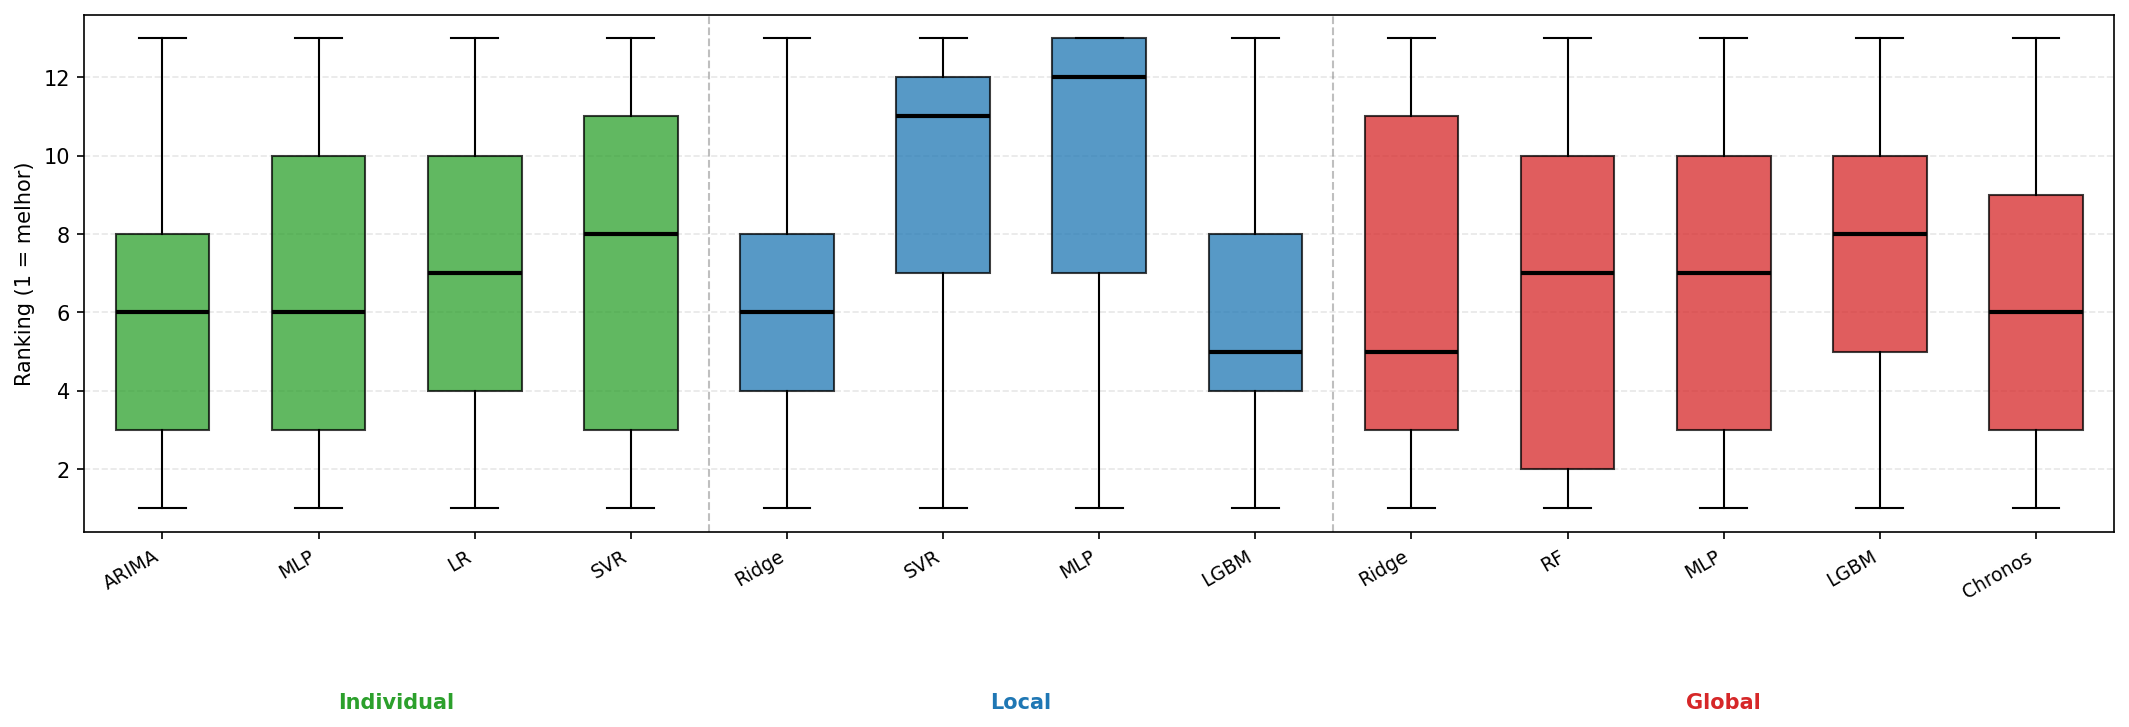
\includegraphics[width=.85\linewidth]{figs/boxplot_paradigmas_receita_todos.png}
\caption{Distribuição do rank baseado em RMSE por modelo, agrupado por abordagem, na previsão das séries de receita.}
\label{fig:boxplot_receita}
\end{figure}

\subsection{Avaliação de desempenho para as séries temporais de despesa}\label{sec:despesa}

A Tabela~\ref{tab:resultados_despesa} apresenta os resultados obtidos pelas abordagens individual, local e global na previsão das séries temporais de despesas. Na abordagem individual, o modelo SVR apresentou o melhor desempenho geral, alcançando os menores RMSE, DP e MAPE, além de ter obtido o maior número de vitórias, sendo o melhor modelo em 7 das 16 séries analisadas (43,8$\%$). Na abordagem local, o SVR também se destacou ao registrar o menor RMSE e a maior frequência de vitórias (31,2$\%$). O modelo Ridge apresentou desempenho próximo, com RMSE de 0,669, mesma porcentagem de vitórias (31,2$\%$) e menor desvio padrão (0,36), enquanto o MLP obteve o menor MAPE da abordagem (49,7$\%$). De modo geral, os resultados indicam que entre os modelos locais, 3 dos 4 apresentaram desempenho relativamente homogêneo nas séries de despesas, com exceção do LightGBM que obteve métricas de erro maiores. Entre os modelos globais, o Chronos alcançou o melhor desempenho em termos de RMSE ($0,447$) e foi o modelo mais vitorioso da abordagem, obtendo o melhor resultado em 9 das 16 séries (56,2\%). Além disso, apresentou o menor MAPE da abordagem global (50,1\%). Os demais modelos globais exibiram desempenhos próximos entre si, com destaque para o LightGBM, que registrou o menor desvio padrão (0,38).

Na análise do ``Melhor'' entre as abordagens, o paradigma global apresentou o melhor desempenho geral, alcançando RMSE de $0,352$ e MAPE de 39,8\%. Em termos de frequência de vitórias, a abordagem global também apresentou o maior percentual (43,8\%), seguida pela individual (37,5\%) e pela local (18,8\%). Esses resultados sugerem que, para as séries de despesa analisadas, os modelos globais foram mais eficazes em capturar padrões compartilhados entre as séries.

\begin{table}[ht]
\centering
\caption{Resultados em termos de RMSE, MAPE e Desvio Padrão (DP) das abordagens individual, local e global para a previsão de séries temporais de receita. Os melhores desempenhos por abordagem estão em negrito. A coluna ``Vitória'' indica a contagem e o percentual de séries em que cada modelo obteve o melhor desempenho dentro de sua respectiva abordagem.}
\label{tab:resultados_despesa}
\footnotesize
\scalebox{0.7}{
\begin{tabular}{clrrrr}
\toprule
\textbf{Abordagem} & \textbf{Modelo} & \textbf{RMSE} & \textbf{DP} & \textbf{MAPE} & \textbf{Vitória} \\
\midrule
\multirow{4}{*}{\textbf{Individual}} 
&ARIMA & 0,845 & 1,35 & 62,9\% & 2~(12,5\%) \\
&MLP   & 0,788 & 0,61 & 48,0\% & 4~(25,0\%) \\
&Ridge & 0,746 & 2,00 & 53,8\% & 3~(18,8\%) \\
&SVR   & \bf 0,691 & \bf 0,59 & \bf 43,3\% & \bf 7~(43,8\%) \\
\cmidrule{2-6}
& Melhor & 0,671 & 0,45 & 43,7\% & 6~(37,5\%) \\
\midrule
\multirow{4}{*}{\textbf{Local}} 
&LightGBM & 0,893 & 0,39 & 59,2\% & 2~(12,5\%) \\
&MLP      & 0,689 & 0,37 & \bf 49,7\% & 4~(25,0\%) \\
&Ridge    & 0,669 & \bf 0,36 & 51,7\% & \bf 5~(31,2\%) \\
&SVR      & \bf 0,608 & \bf 0,36 & 52,6\% & \bf 5~(31,2\%) \\
\cmidrule{2-6}
& Melhor & 0,547 & 0,34 & 44,1\% & 3~(18,8\%) \\
\midrule
\multirow{5}{*}{\textbf{Global}} 
&Chronos  & \bf 0,447 & 0,83 & \bf 50,1\% & \bf 9~(56,2\%) \\
&LightGBM & 0,641 & \bf 0,38 & 58,0\% & 2~(12,5\%) \\
&MLP      & 0,593 & 0,61 & 62,5\% & 1~(6,2\%) \\
&RF       & 0,680 & 0,40 & 55,7\% & 2~(12,5\%) \\
&Ridge    & 0,589 & 0,55 & 71,2\% & 2~(12,5\%) \\
\cmidrule{2-6}
& Melhor & 0,352 & 0,42 & 39,8\% & 7~(43,8\%) \\
\bottomrule
\end{tabular}
}
\end{table}


Os resultados para as séries de despesa, sintetizados na Tabela~\ref{tab:rankings_despesa} e na Figura~\ref{fig:boxplot_despesa}, revelam uma clara superioridade da abordagem Global, com o modelo Chronos liderando tanto o ranking médio (4,81) quanto o percentual de vitórias (25$\%$). Diferente do observado nas séries de receita, a abordagem global demonstrou maior consistência, ocupando quatro das cinco primeiras posições do ranking. O SVR individual destacou-se como o segundo melhor modelo (6,19), apresentando-se como a alternativa mais robusta fora do paradigma global, enquanto o LightGBM local registrou o desempenho médio mais baixo da amostra ($8,88$). O boxplot confirma essa tendência, evidenciando que a abordagem global, liderada pelo Chronos, obteve a melhor mediana. 

\begin{table}[ht]
\centering
\caption{Ranking de Desempenho baseado no RMSE: posicionamento médio e \% de vitórias por modelo nas séries temporais de despesa. Os resultados estão ordenados pelo rank médio.}
\label{tab:rankings_despesa}
\footnotesize
\scalebox{0.7}{
\begin{tabular}{llcc}
\toprule
\textbf{Abordagem} & \textbf{Modelo} & \textbf{Rank} & \textbf{Vitória~(\%)} \\
\midrule
Global     & Chronos   & 4,81 & 25,0 \\
Individual & SVR       & 6,19 & 12,5 \\
Global     & RF        & 6,25 &  6,2 \\
Global     & LightGBM  & 6,44 &  6,2 \\
Local      & Ridge     & 6,50 &  6,2 \\
Global     & Ridge     & 6,75 &  0,0 \\
Individual & Ridge     & 6,81 &  6,2 \\
Individual & MLP       & 6,81 &  6,2 \\
Local      & MLP       & 7,12 &  0,0 \\
Local      & SVR       & 7,38 &  6,2 \\
Global     & MLP       & 8,38 &  6,2 \\
Individual & ARIMA     & 8,69 & 12,5 \\
Local      & LightGBM  & 8,88 &  6,2 \\
\bottomrule
\end{tabular}
}
\end{table}

\begin{figure}[ht]
\centering
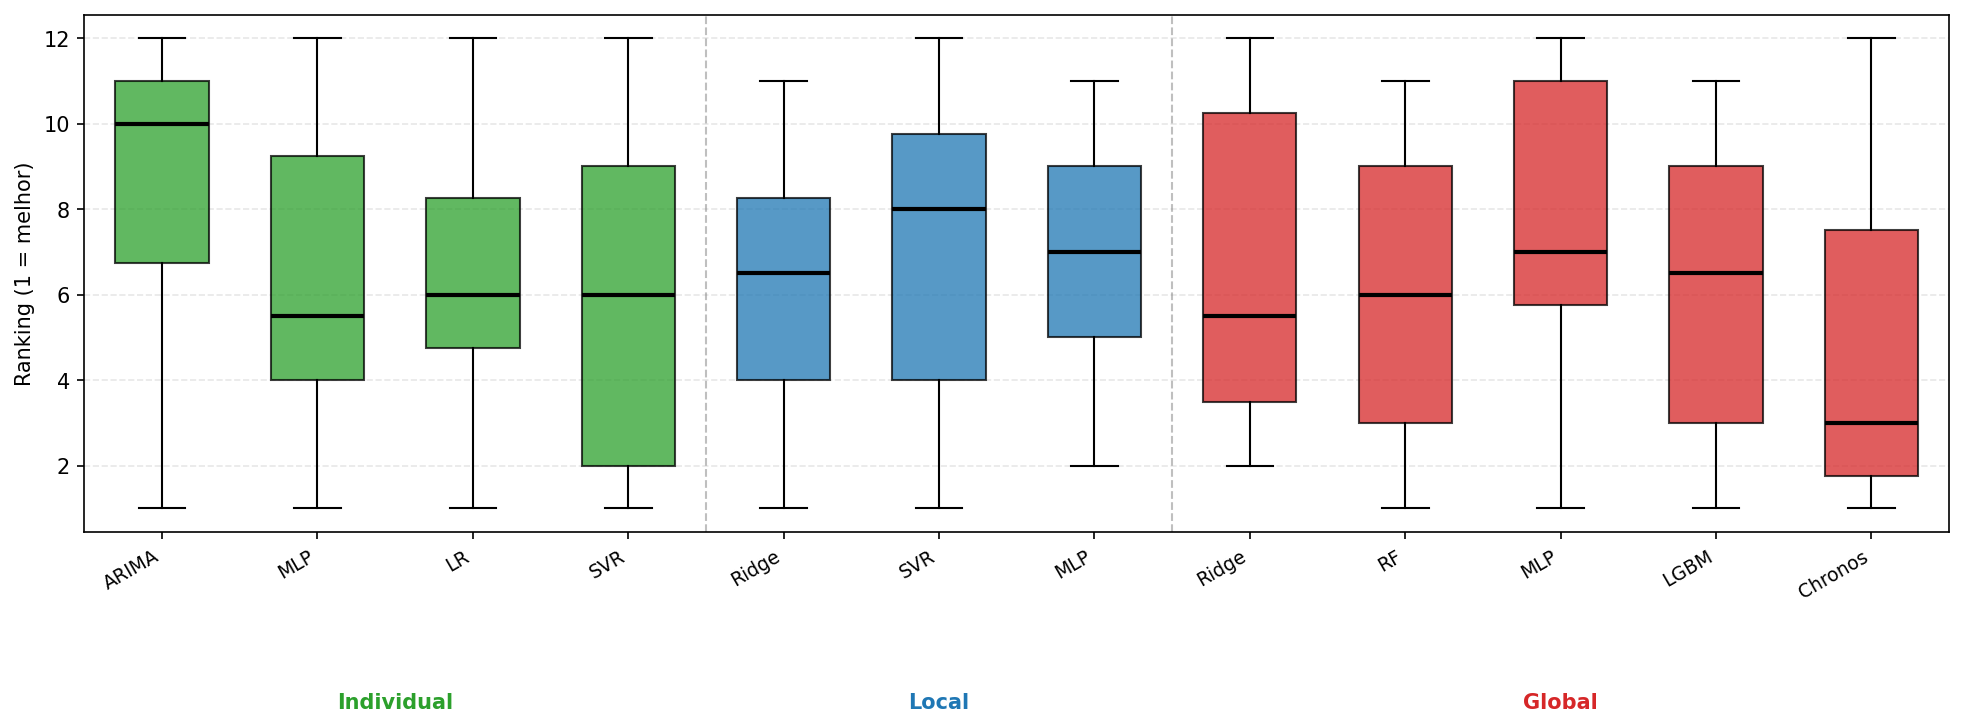
\includegraphics[width=.85\linewidth]{figs/boxplot_paradigmas_despesa_todos.png}
\caption{Distribuição do RMSE por modelo, agrupado por abordagem, na previsão das séries de despesa.}
\label{fig:boxplot_despesa}
\end{figure}

%% ─── 6. Conclusões ───────────────────────────────────────────────────────────
\section{Conclusões}
\label{sec:conclusao}

Este trabalho investigou o desempenho dos paradigmas de aprendizado individual, local e global na previsão de receitas e despesas públicas, utilizando uma gama de modelos que incluiu desde abordagens estatísticas clássicas até modelos de fundação. Os resultados demonstraram que não existe uma superioridade universal de um único paradigma, mas sim uma dependência direta das características das séries fiscais. Para as receitas, as abordagens individual e local mostraram-se altamente competitivas, enquanto nas despesas a abordagem global, liderada pelo modelo Chronos, apresentou maior consistência e robustez. Em resumo, os achados evidenciam que a integração de modelos de fundação com treinamentos locais e globais oferece o caminho mais promissor para lidar com a heterogeneidade das finanças públicas, contribuindo para previsões mais precisas que podem fortalecer o planejamento governamental e a sustentabilidade fiscal.

Como trabalhos futuros, destacam-se a incorporação de variáveis exógenas e o desenvolvimento de estratégias de combinação que explorem a complementaridade entre modelos de fundação e modelos treinados sobre os próprios dados~\cite{petropoulos2022forecasting}.

%% ─── Referências ─────────────────────────────────────────────────────────────
\bibliographystyle{sbc}
\bibliography{referencias_eniac}

\end{document}